\documentclass{article}
\usepackage[utf8]{inputenc}
\usepackage{graphicx}
\usepackage{mathtools} 
\usepackage{textcomp}
\usepackage{titling}
\usepackage{subfig}
\usepackage{amsmath}
\usepackage[parfill]{parskip}
\usepackage{xcolor}
\definecolor{LightGray}{gray}{0.9}
\usepackage{titlesec}
\setcounter{secnumdepth}{4}
\usepackage[a4paper,left=1cm,right=1cm,top=1cm,bottom=1.5cm,]{geometry}
\usepackage{eqparbox}
\usepackage{enumitem}

\title{\vspace{-2cm} MA2101 L4 - Jordan Canonical Form}
\date{\vspace{-5ex}}

\begin{document}
\maketitle

\section{Jordan Block}
\begin{itemize}
    \item Suppose $\lambda$ is any scalar. 
    \item Then a \textit{Jordan block} of size \textit{m} is simply an (\textit{m}$\times$\textit{m}) matrix of the form \dots
    \begin{figure}[htp]%
        \centering
        \subfloat[\centering Generic form]{{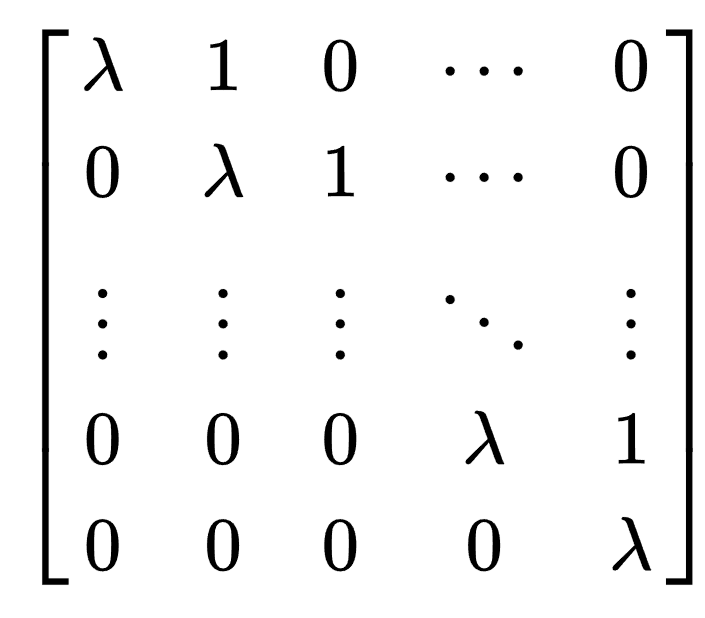
\includegraphics[width=3cm]{S1/jordanBlock.PNG}}}% 
        \qquad
        \subfloat[\centering \textit{m}=4]{{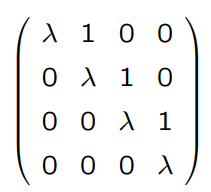
\includegraphics[width=3cm]{S1/jordanBlock4.PNG}}}% 
        \caption{Jordan block structure}%
    \end{figure}
\end{itemize}

Note that a (\textit{1}$\times$\textit{1}) Jordan block is simply a \textbf{scalar}

\subsection{Properties of the Jordan block}
\begin{large}
    \underline{CLAIM}: Every Jordan block has only \textbf{one} eigenspace , and it is \textbf{one-dimensional}
\end{large}

\begin{enumerate}[label*=\arabic*.]
    \item Let's prove why the Jordan block has only one eigenspace. 
            This is equivalent to saying that the Jordan block has only one eigenvalue (which already seems true by definition).
            \begin{enumerate}[label*=\arabic*.]
                \item Suppose we rewrite the diagonal $\lambda$'s of the generic Jordan block in Fig1 as $\lambda_{1}$
                \item Consider the \textit{characteristic polynomial} $p_{A}$ of the 'rewritten' generic Jordan block \textit{A}, defined as $p_{A}(\lambda) = det(A - \lambda I)$
                \item We know that the determinant of an upper triangular matrix is the product of the \textbf{main} diagonal entries,
                        therefore $p_{A} = (\lambda_{1}-\lambda)^{m}$, supposing that $A$ is an \textit{m}$\times$\textit{m} square matrix
                \item Thus, we have that the \textbf{only} eigenvalue is $\lambda_{1}$
            \end{enumerate}
    \item Let's prove that the eigenspace corresponding to the eigenvalue $\lambda_{1}$ is one-dimensional
            \begin{enumerate}[label*=\arabic*.]
                \item The eigenspace is defined as the nullspace of (\textit{A}-$\lambda$I), since we are trying to solve $(A-\lambda I)v = 0$
                \item Solving for \textit{v} above, we get $v = (1,0,\dots,0)^{T}$
                \item Span of \textit{v} is one dimensional, therefore the eigenspace must be one dimensional
            \end{enumerate}
\end{enumerate}

\vspace{0.25cm}
Intuitively, the presence of Jordan blocks signals to us that we \textbf{do not have enough eigenvectors} to form a basis -- which is why we cannot diagonalise

\section{Jordan Basis}
A \textit{Jordan basis} is a basis st. the matrix (wrt to this Jordan basis) of some operator T consists of \textit{Jordan blocks} $J_{i}$

\begin{minipage}{0.45\linewidth}
    \centering
    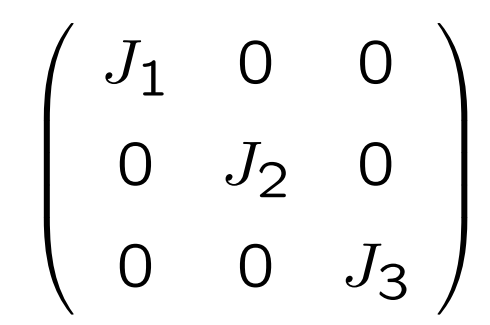
\includegraphics[width=5cm]{S1/jordanBasis1.PNG}
    \captionsetup{justification=centering}
    \captionof{figure}{Abstracted view\\~\\
                       Since the entire matrix is upper triangular (and so are the Jordan blocks $J_{i}$),
                       the eigenvalues of the matrix are along the \textbf{main} diagonal}
\end{minipage}%
\hfill
\begin{minipage}{0.55\linewidth}
    \centering
    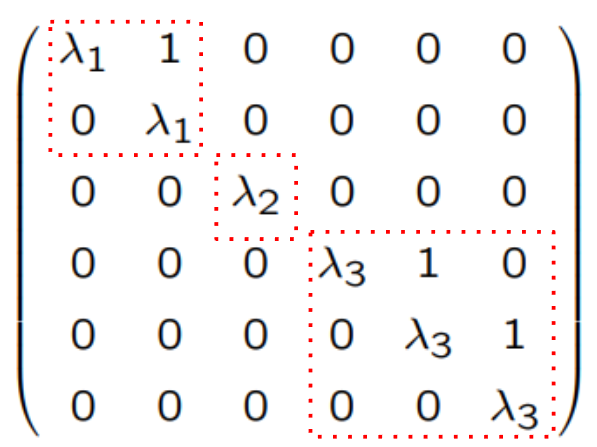
\includegraphics[width=5cm]{S1/jordanBasis2.PNG}
    \captionsetup{justification=centering}
    \captionof{figure}{3 Jordan blocks in a \textit{6}$\times$\textit{6} matrix\\~\\
                        Ordering is not unique, it depends on how we order the basis vectors. Furthermore, the $\lambda_{i}$'s do not have to be distinct}
\end{minipage}%

\newpage
\subsection{Properties of the Jordan basis}
\begin{large}
    \underline{CLAIM}: Every operator on a \textbf{complex} vector space has a Jordan basis
\end{large}

\begin{itemize}
    \item This Jordan basis is \textbf{unique}, disregarding the possibility of changing the ordering of the basis.
            This is because a basis is strictly speaking an ordered set, therefore changing the ordering is changing the basis.
    \item Intuitively, this is saying that every \textbf{complex} matrix \textit{A} 
            is \textit{similar} to a matrix \textit{B} that is built up from Jordan blocks, 
            similar in the sense that $A = P^{-1}BP$ for some \textit{change-of-basis} matrix \textit{P}
\end{itemize}

Proof is skipped for this, it is quite involved.

\section{Jordan Canonical Form}
When an operator is represented by a matrix wrt a Jordan basis, we say the matrix is in \textit{Jordan Canonical Form}.

\begin{enumerate}[label*=\arabic*.]
    \item Suppose we agree that an upper triangular matrix \textit{A} of the form
        $
            \left(
            \begin{array}{ccccc}
            \lambda_{1}                              \\
            & \lambda_{2}     &   & \textbf{\huge *} \\
            &                 & \ddots               \\
            & \textbf{\huge0} &   & \lambda_{n-1}    \\
            &                 &   &   & \lambda_{n}
            \end{array}
            \right)_{\left\{ b_{1}, b_{2}, \dots, b_{n} \right\}}
        $ 

        has the property that $Ab_{i} = \alpha_{1}b_{1} + \alpha_{2}b_{2} + \dots + \lambda_{i}b_{i}$. (This is taken at face-value, it is not simple to prove.)
        \begin{enumerate}[label*=\arabic*.]
            \item Intuitively, every basis vector $b_{i}$ is mapped to a linear combination of it's 'lower' basis vectors $b_{j}, j \le i$
            \item We can see this from the matrix structure. For some $i^{th}$ column, we have that the rows $\left\{ A_{1i}, A_{2i}, \dots, A_{ii} \right\}$ are non-zero.
                    Therefore, this means that the $i^{th}$ basis vector is mapped to a linear combination of the previous \textit{(i-1)} basis vectors.
        \end{enumerate}
    \item Suppose now that we have the Jordan Canonical Form matrix as seen below.
    
    \begin{minipage}{\linewidth}
        \centering
        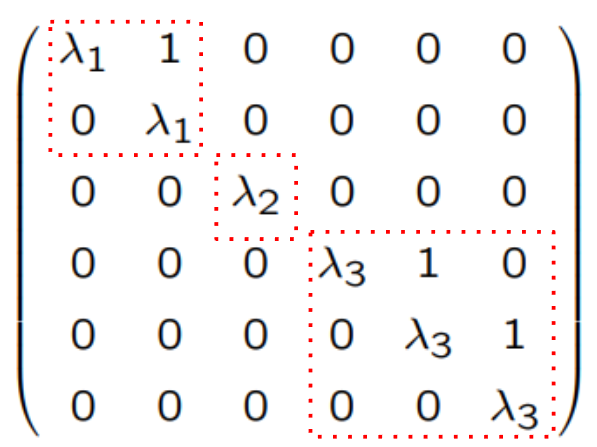
\includegraphics[width=5cm]{S1/jordanBasis2.PNG}
        \captionsetup{justification=centering}
        \captionof{figure}{JCF Matrix}
    \end{minipage}%

    \begin{enumerate}[label*=\arabic*.]
        \item Observe some $i^{th}$ column. We have that there are \textbf{at most two} non-zero entries, therefore every basis vector is mapped to a linear combination
                of \textbf{at most two} basis vectors (including the original basis vector).
    \end{enumerate}
\end{enumerate}

\subsection{Properties of the Jordan Canonical Form}

\subsubsection{Multiplicity of $\lambda$}

\begin{enumerate}[label*=\arabic*.]
    \item Let $\lambda$ be an eigenvalue of a linear transformation
    \item We define the \textit{multiplicity} of $\lambda$ as the sum of sizes of the Jordan blocks corresponding to that eigenvalue
        \begin{enumerate}[label*=\arabic*.]
            \item Simply put, multiplicity is the total number of times a given eigenvalue occurs down the diagonal
        \end{enumerate}
\end{enumerate}


\subsubsection{Characteristic polynomial of \textit{T}}
\begin{enumerate}[label*=\arabic*.]
    \item Let $\lambda_{1}, \lambda_{2}, \dots$ be the eigenvalues of a linear operator \textit{T}
    \item Let $m_{i}$ be the multiplicity of some eigenvalue $\lambda_{i}$
    \item We define the \textit{characteristic polynomial of T} as the polynomial $\mathcal{X}_{T}(x) = (x-\lambda_{1})^{m_{1}} \times (x-\lambda_{2})^{m_{2}} \times \dots$
        \begin{enumerate}[label*=\arabic*.]
            \item By definition, we have that $\forall i,\ \mathcal{X}_{T}(\lambda_{i}) = 0$
            \item However, a more surprising claim is the \textit{Cayley-Hamilton Theorem} in the subsequent section
        \end{enumerate}
\end{enumerate}

\newpage
\section{Cayley-Hamilton Theorem}
\subsection{Definiton of Cayley-Hamilton Theorem}
Cayley-Hamilton Theorem states that $\mathcal{X}_{T}(T) = \textbf{0}$; (Note that \textbf{0} is the zero matrix)

\begin{itemize}
    \item Simply put, it says that the transformation (equivalently, it's matrix relative to any basis) satisfies it's own characteristic equation
    \item Bear in mind that any matrix \textit{similar} to the given one has the same eigenvalues (a property of similarity). Therefore, it must also satisfy any polynomial equation satisfied by the original matrix.
\end{itemize}

\subsection{Proving Cayley-Hamilton Theorem}
\subsubsection{Proving CHT - Diagonal matrix}
\begin{figure}[htp]
    \centering
    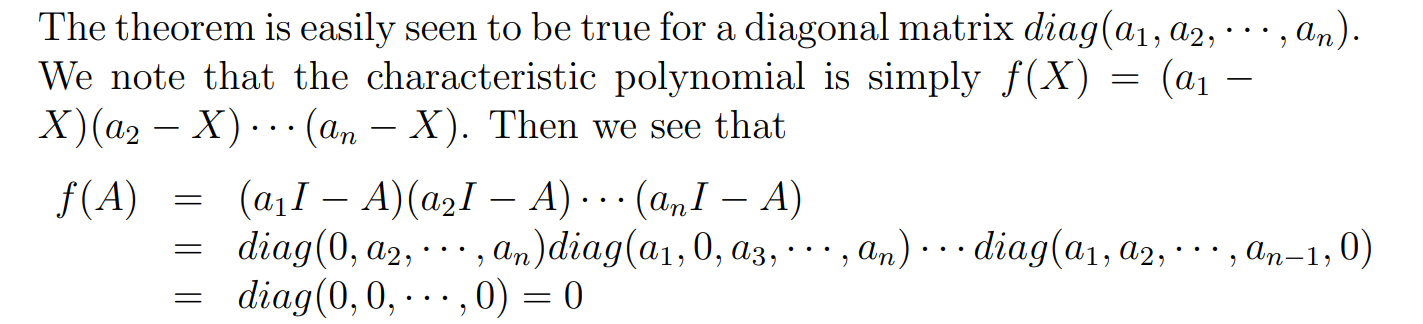
\includegraphics[width=15cm, scale=1]{S4/cayleyHamilton_diagonal.PNG}
\end{figure}

\subsubsection{Proving CHT - Diagonalizable matrix}
\begin{enumerate}
    \item Suppose we have a \textit{diagonalizable} matrix A
    \item By definition of diagonalizablity, $A = PDP^{-1}$
    \item Therefore, $(A-\lambda I) = (PAP^{-1} - \lambda I) = P(A-\lambda I)P^{-1}$
    \item det$\Bigl( P(A-\lambda I)P^{-1} \Bigr)$ = det(P) * det(A-$\lambda I$) * det($P^{-1}$) = det(A-$\lambda I$)
    \item Therefore, we observe that \textit{diagonalizable} matrix A and \textit{diagonal} matrix D have the same characteristic polynomial
\end{enumerate}

\subsubsection{Proving CHT - Non-diagonalizable matrix (Using JCF)}
The difficult part is in proving CHT for non-diagonalizable matrices (if we can prove this, then we can prove CHT is true for any general square matrix).

Tutorial question uses \textit{Analysis} method of proving. Here, we will use JCF to prove.

\vspace{0.5cm}
\begin{enumerate}[label*=\arabic*.]
    \item Assume that we have used \textit{similarity} to turn some square matrix into it's Jordan Canonical Form
    \item Let's use a concrete example for this case. Consider the Jordan block \textit{B} we saw in the \textit{6}$\times$\textit{6} matrix of Fig3
            \[
                B=
                \begin{bmatrix}
                    \lambda_{3} & 1 & 0 \\
                    0 & \lambda_{3} & 1 \\
                    0 & 0 & \lambda_{3}
                \end{bmatrix}
            \] 
\end{enumerate}


TO BE DONE.... MA2101 L4 Pg39

$\frac{1}{1+e^{-x}} \xrightarrow{\text{Translate right}} \frac{1}{1+e^{-(x-3)}} \xrightarrow{\text{Horizontal Stretch}} \frac{1}{1+e^{-(\frac{6}{256}x-3)}} \xrightarrow{\text{Vertical Stretch}} \frac{256}{1+e^{-(\frac{6}{256}x-3)}}$










\end{document}